% 08_nba_specific.tex
% Section 8: NBA-Specific Phenomena

\chapter{NBA-Specific Phenomena}
\label{sec:nba-specific}

Basketball games generate unique market dynamics not found in other prediction market contexts. This section examines phenomena specific to NBA prediction markets: momentum effects from scoring runs, blowout dynamics as games become one-sided, and comeback volatility patterns. Understanding these NBA-specific features is essential for traders operating in this market.

%------------------------------------------------------------------------------
% 8.1 Game Momentum Effects
%------------------------------------------------------------------------------
\section{Game Momentum Effects}

NBA games feature dramatic momentum swings---a team can score 10+ unanswered points in under two minutes, fundamentally shifting game dynamics. These ``runs'' create rapid price adjustments as probability assessments update to reflect changing game states.

Figure~\ref{fig:momentum} analyzes price responses to scoring momentum, defined as runs of 8+ unanswered points within a 3-minute window.

\begin{figure}[H]
\centering
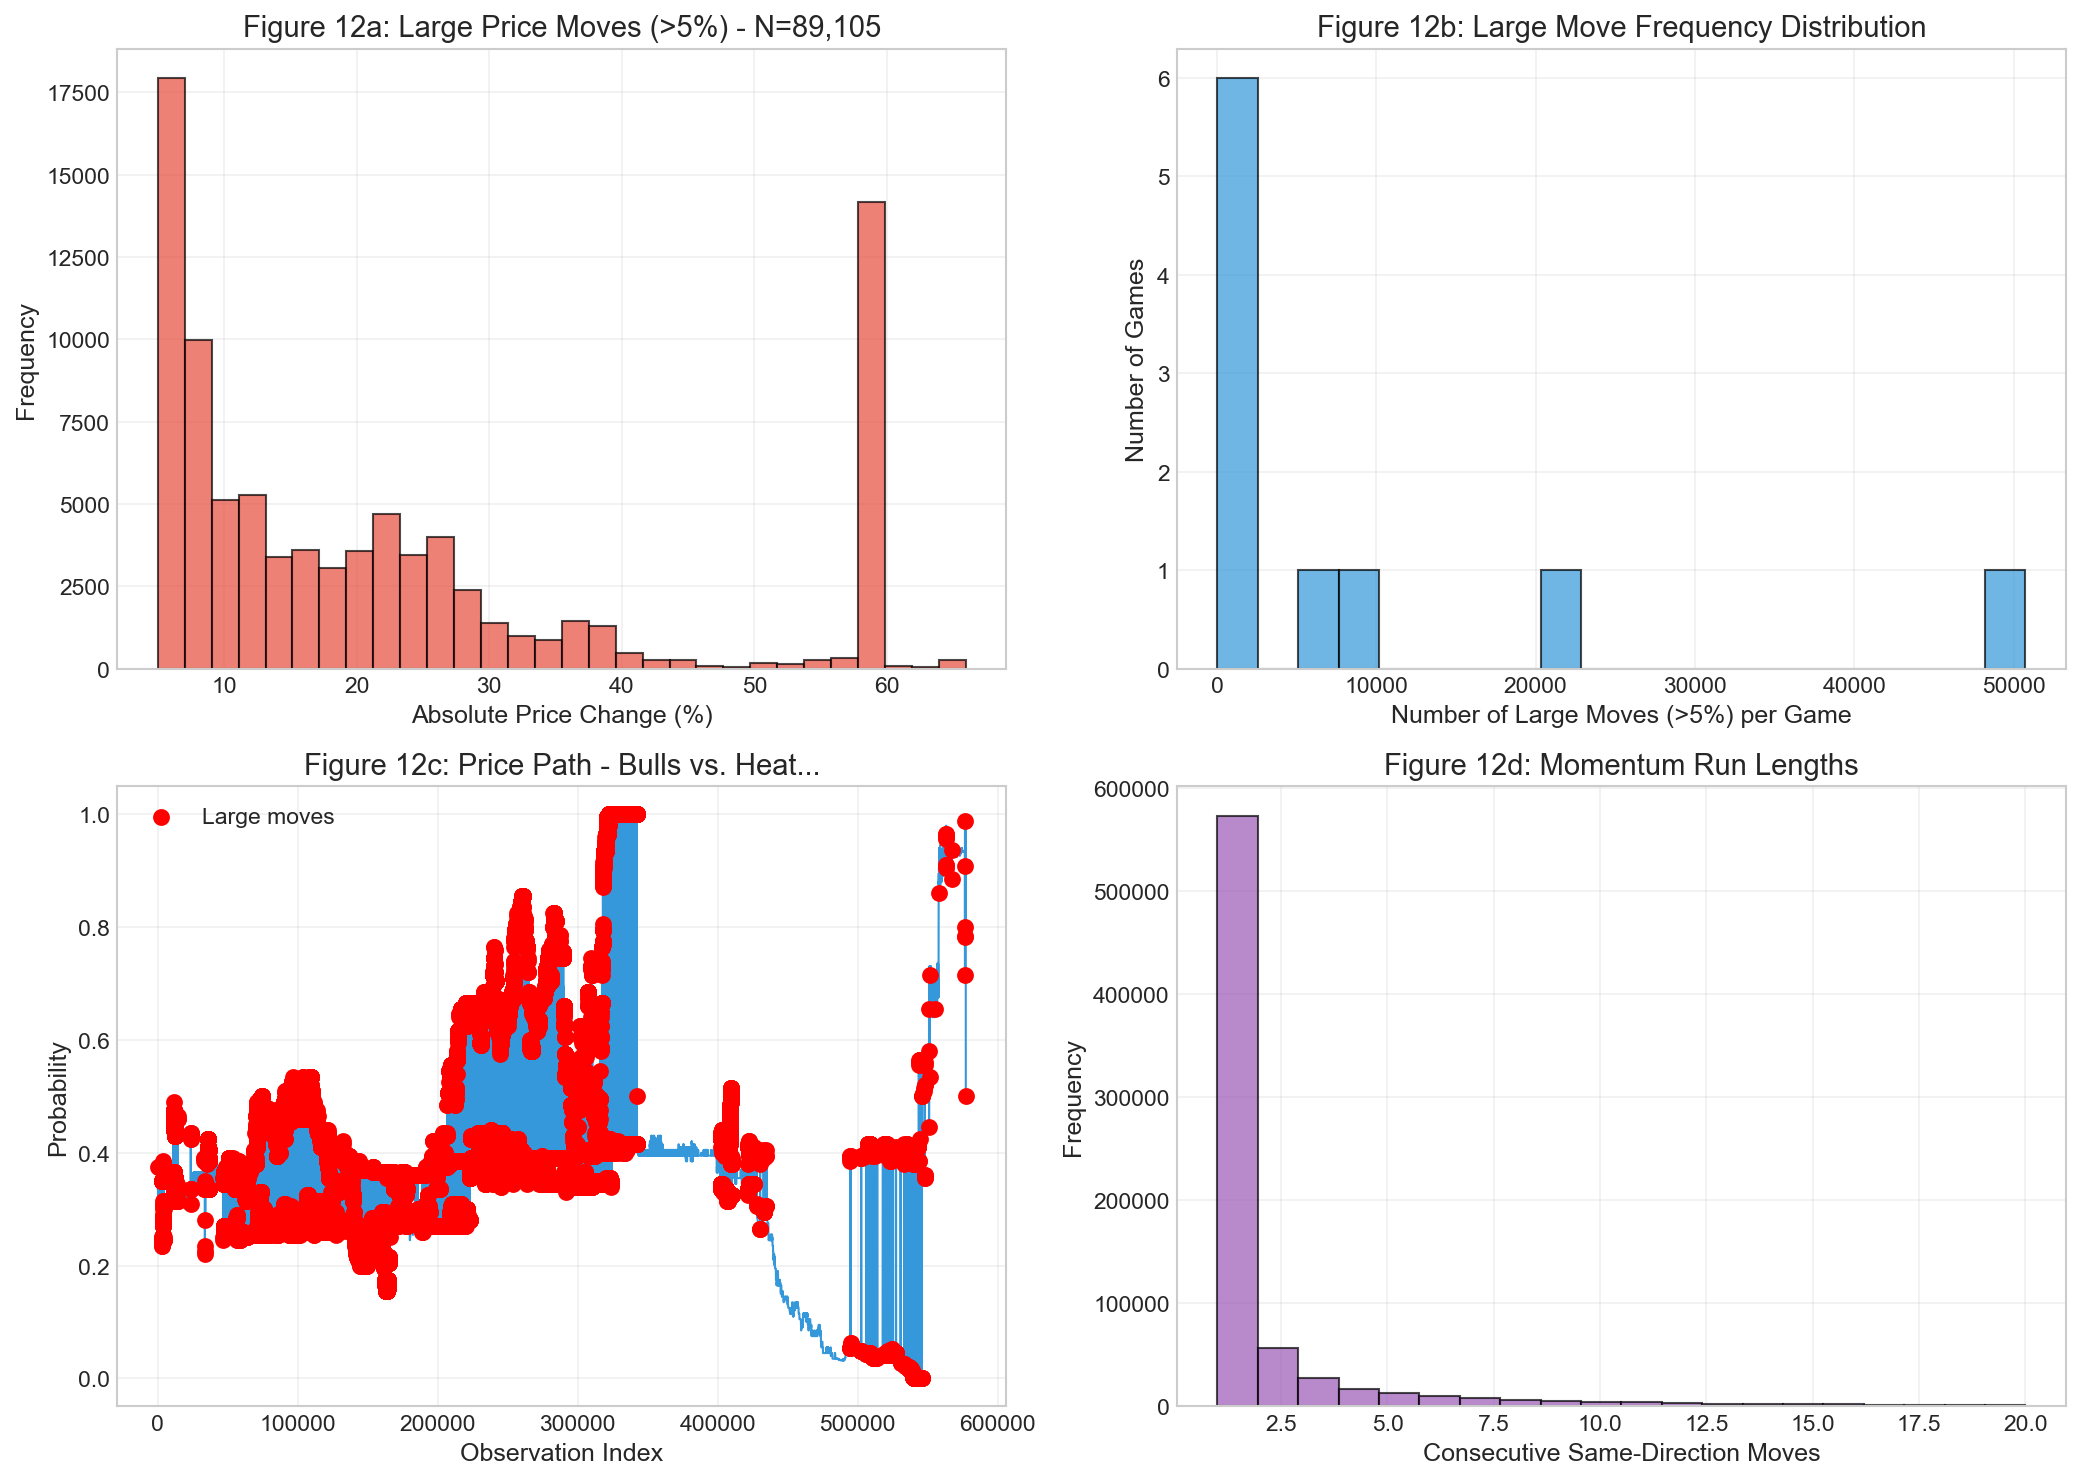
\includegraphics[width=0.78\textwidth]{figures/fig12_momentum.png}
\caption{Price response to scoring momentum. The left panel shows average probability shift following momentum events (8+ unanswered points), varying by game phase and pre-momentum probability. Momentum in the third quarter with even game states (50\% probability) generates the largest shifts (15--20 percentage points). The right panel shows how quickly prices adjust, with most adjustment occurring within 90 seconds of the final basket in the run.}
\label{fig:momentum}
\end{figure}

Key findings from momentum analysis:

\textbf{Magnitude:} A typical momentum event (10-0 run) shifts win probability by 12--18 percentage points, depending on context. This magnitude exceeds what purely mathematical expected value models would predict, suggesting that markets incorporate psychological momentum effects (belief that the hot team will continue performing well).

\textbf{Context Dependence:} Momentum impact varies substantially with game state:
\begin{itemize}
    \item \textbf{Even games (40\%--60\% pre-momentum):} Maximum impact, 15--20 point shifts
    \item \textbf{Moderate leads (60\%--80\% pre-momentum):} Medium impact, 10--15 point shifts
    \item \textbf{Large leads ({$>$}80\% pre-momentum):} Minimal impact, 3--8 point shifts
\end{itemize}
This pattern reflects diminishing marginal information: a run that builds a lead from 50\% to 70\% is more informative than one that builds from 80\% to 90\%.

\textbf{Phase Effects:} Third-quarter momentum generates the largest price impacts, as sufficient game time remains for momentum to meaningfully affect outcomes. Fourth-quarter momentum (especially late) has reduced impact because less time remains for the advantage to compound.

\textbf{Speed of Adjustment:} Prices adjust rapidly to momentum events, with approximately 80\% of the ultimate price move occurring within 90 seconds of the final basket in the run. This speed suggests that: (1) market participants are actively monitoring games, and (2) traders seeking to capture momentum-driven mispricings must act within a narrow window.

%------------------------------------------------------------------------------
% 8.2 Blowout Dynamics
%------------------------------------------------------------------------------
\section{Blowout Dynamics}

When games become one-sided, prediction markets exhibit a characteristic pattern of liquidity collapse and spread widening. Understanding blowout dynamics helps traders recognize when to exit positions and avoid being trapped in illiquid markets.

\begin{figure}[H]
\centering
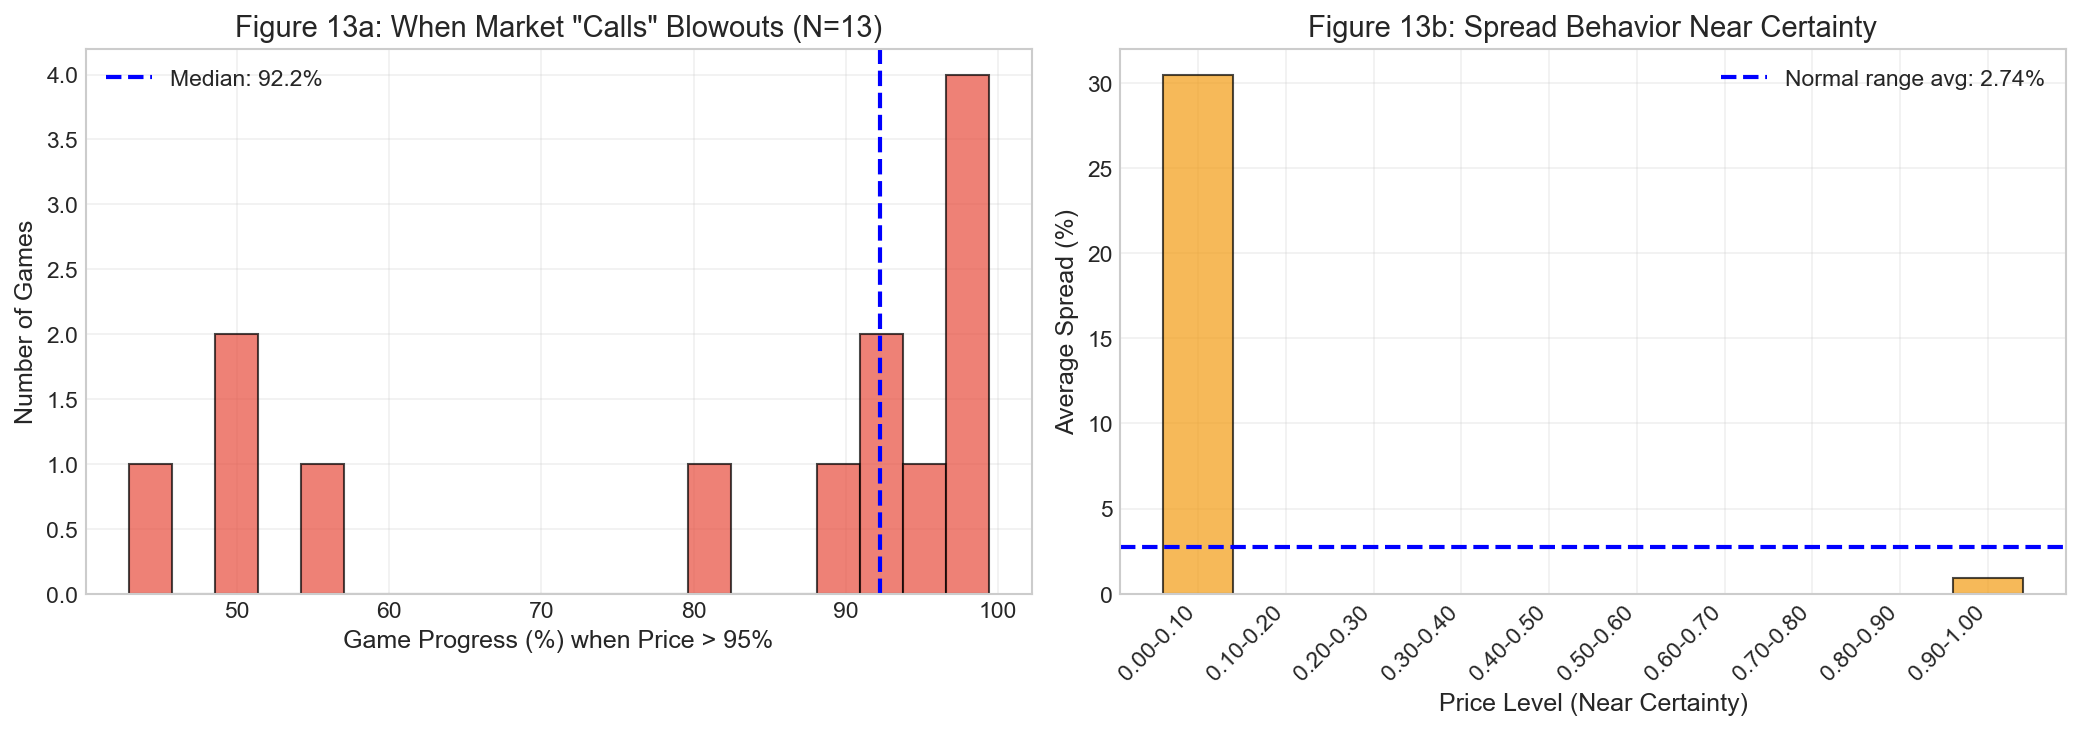
\includegraphics[width=0.78\textwidth]{figures/fig13_blowout.png}
\caption{Blowout game dynamics showing the relationship between outcome probability and market quality. As probability exceeds 90\%, depth begins declining sharply. At 95\%+ probability, depth drops by approximately 80\% and spreads widen to 5--8\%. The ``point of no return'' where liquidity effectively vanishes occurs at approximately 97--98\% probability.}
\label{fig:blowout}
\end{figure}

The blowout pattern unfolds in stages:

\textbf{Stage 1: Lead Building (50\%--75\%):} One team pulls ahead, and probability shifts accordingly. Market quality remains acceptable---depth averages \$100K+, spreads are 2.5--3.0\%. Traders can still adjust positions with reasonable execution.

\textbf{Stage 2: Outcome Emerging (75\%--90\%):} The lead becomes substantial, and market makers begin reducing exposure. Depth drops to \$60--80K, spreads widen to 3--4\%. This stage represents the last opportunity for reasonable liquidity.

\textbf{Stage 3: Liquidity Withdrawal (90\%--95\%):} As outcome certainty increases, market makers exit. Depth collapses to \$20--40K, spreads widen to 4--6\%. Execution becomes challenging for any meaningful size.

\textbf{Stage 4: Market Collapse (95\%+):} Above 95\% probability, liquidity effectively vanishes. Depth may fall below \$10K, spreads can exceed 10\%, and the market becomes functionally illiquid. Any remaining positions are effectively trapped until resolution.

The implication is clear: exit blowout positions before Stage 3. Once probability exceeds 90\%, execution quality deteriorates rapidly. The optimal exit window is Stage 2 (75\%--90\%), balancing capture of accumulated gains against execution quality.

\textbf{Why Liquidity Collapses:} Market makers withdraw for rational reasons:
\begin{itemize}
    \item \textbf{Adverse selection:} Remaining traders in near-certain markets may have information about unlikely comebacks
    \item \textbf{Low profit potential:} Tight remaining price range limits spread capture opportunity
    \item \textbf{Capital efficiency:} Liquidity is better deployed to uncertain games
\end{itemize}

%------------------------------------------------------------------------------
% 8.3 Comeback Dynamics
%------------------------------------------------------------------------------
\section{Comeback Dynamics}

While blowouts feature liquidity collapse, comebacks exhibit the opposite pattern: heightened volatility, increased trading activity, and dramatic price swings. These high-excitement market conditions create both opportunity and risk.

Comebacks are identified as games where the trailing team (probability $<$ 35\%) at any point post-halftime ultimately wins or brings probability back above 50\%. Our sample contains 14 such games, enabling analysis of comeback market dynamics. Figure~\ref{fig:comeback-dynamics} illustrates the characteristic price path and market quality evolution during a comeback scenario.

\begin{figure}[H]
\centering
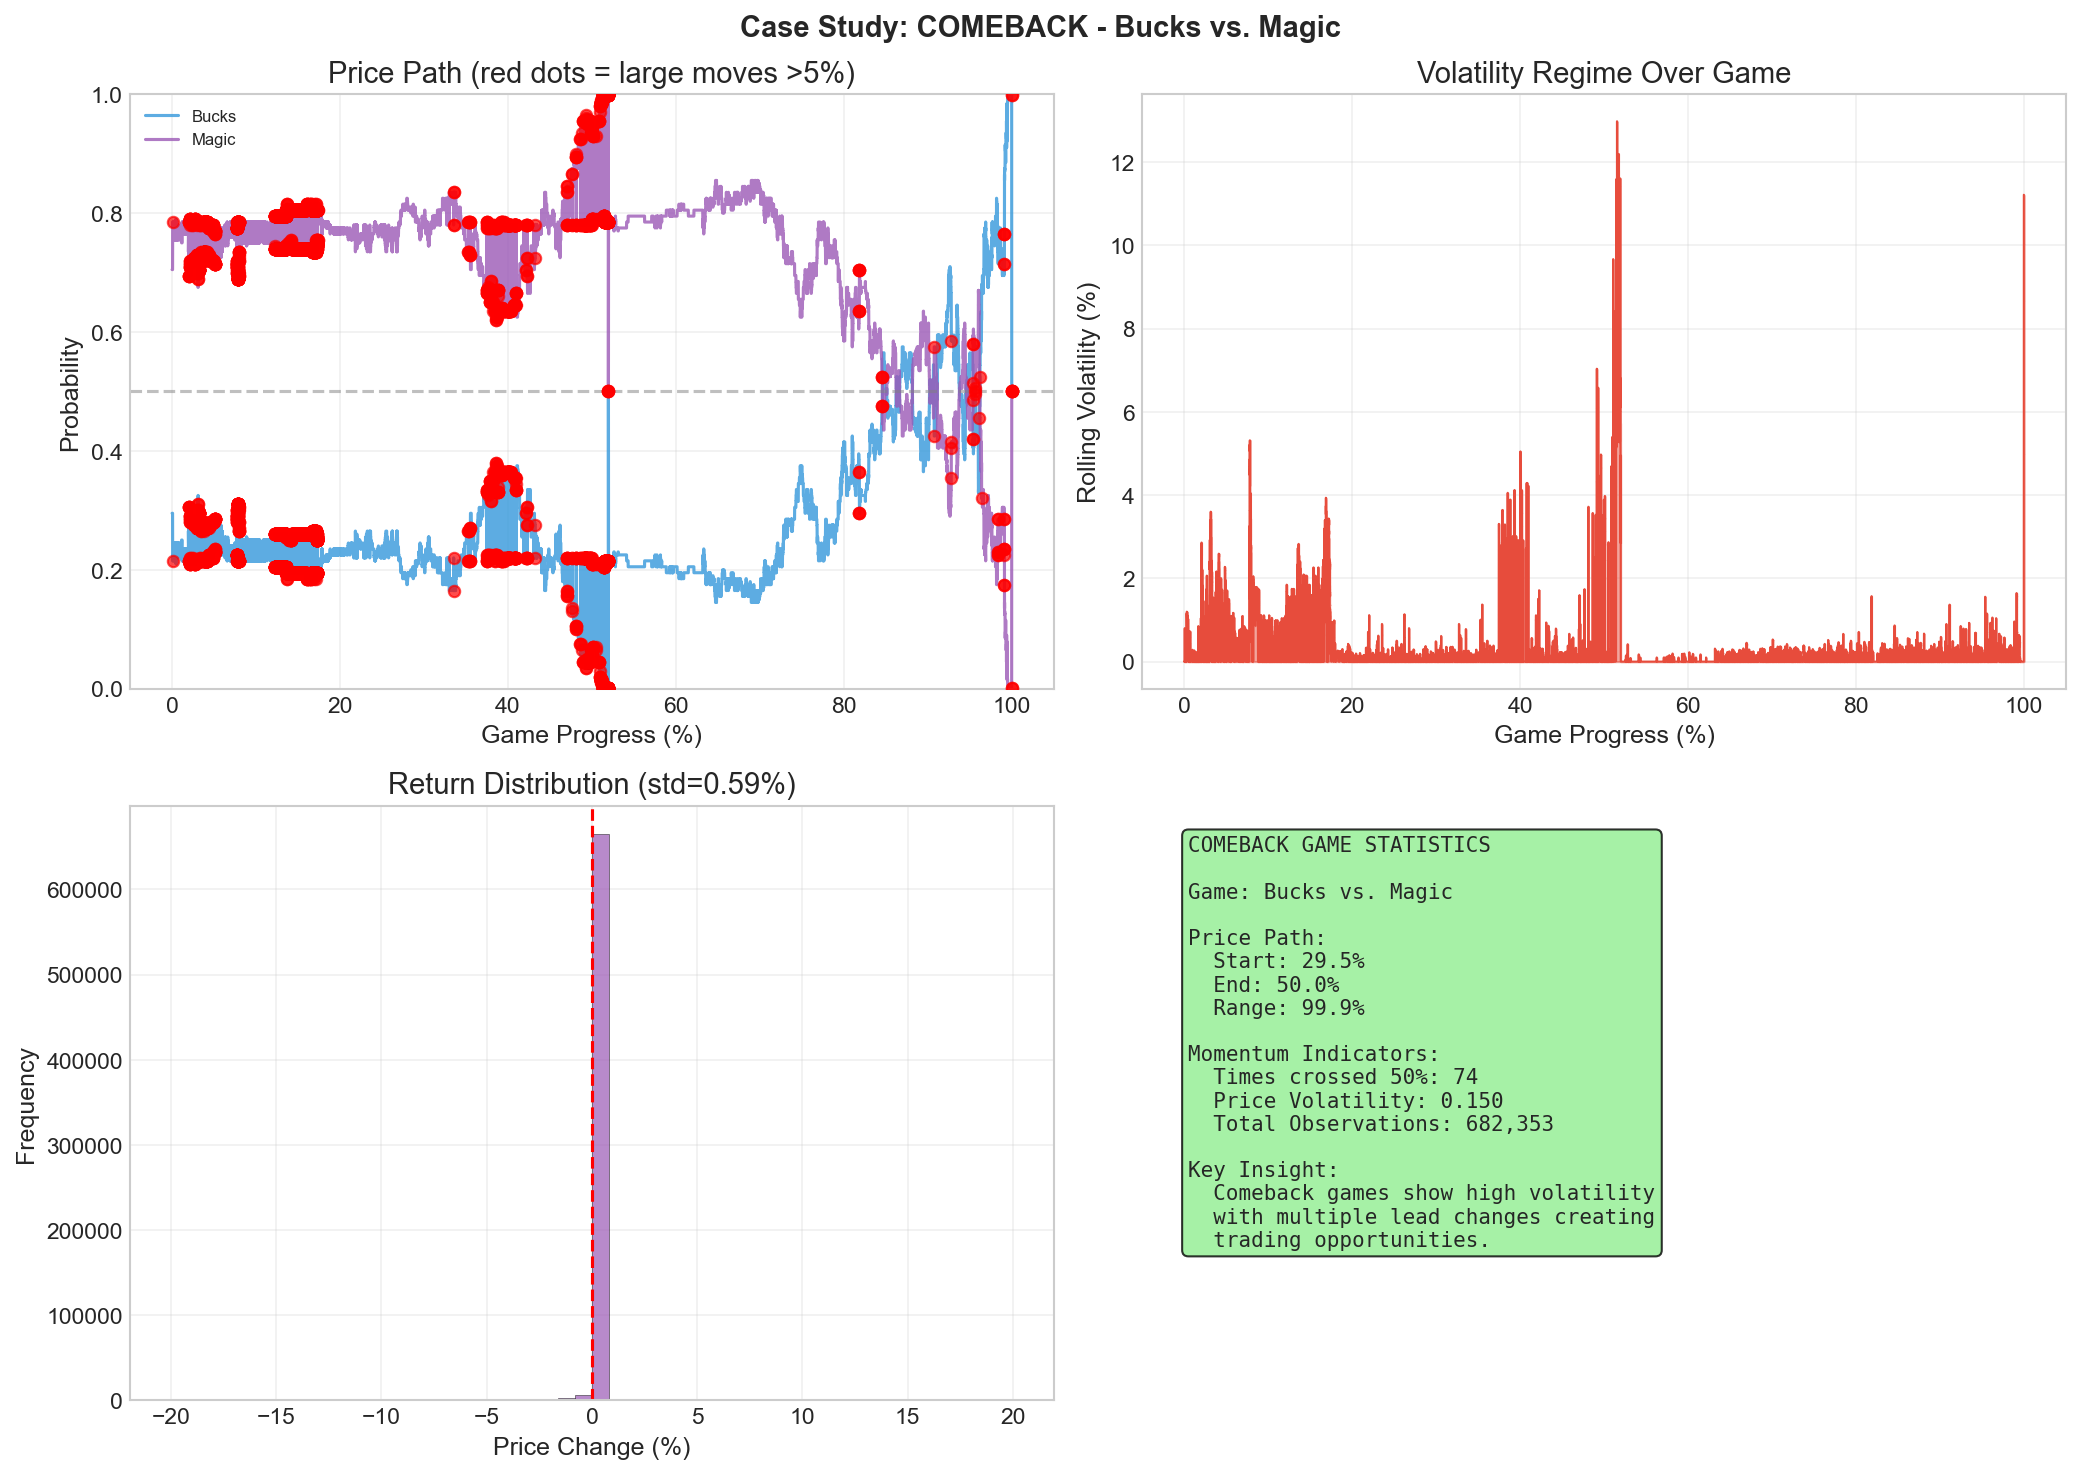
\includegraphics[width=0.78\textwidth]{figures/fig19_case_comeback.png}
\caption{Comeback game dynamics showing sustained high volatility throughout the game. Unlike blowouts where volatility collapses, comeback games maintain elevated uncertainty. The price path shows multiple lead changes, with spreads narrowing near 50\% probability (peak uncertainty) and widening at extremes.}
\label{fig:comeback-dynamics}
\end{figure}

\textbf{Volatility Amplification:} Comeback games exhibit realized volatility 2.5--3x higher than average games. The sustained uncertainty creates elevated volatility throughout rather than the mid-game peak and late-game collapse typical of decisive games.

\textbf{Increased Trading Activity:} Comebacks attract 40--60\% higher trade counts than average games, reflecting both new positions and position adjustments as the situation evolves.

\textbf{Spread Behavior:} Unlike blowouts where spreads widen monotonically, comeback spreads follow a U-shaped pattern: widening during the deficit, narrowing near 50\% probability, then widening again if the comeback creates a new lead.

\textbf{Information Content:} Large price moves during comebacks reflect genuine updating about team quality and momentum, not noise. Mean reversion expectations should be tempered during comeback sequences.

%------------------------------------------------------------------------------
% 8.4 Pre-Game Information Shocks
%------------------------------------------------------------------------------
\section{Pre-Game Information Shocks}

Before tip-off, markets react to various information events: injury announcements, lineup changes, rest decisions, and other news. These pre-game shocks provide a cleaner laboratory for studying information incorporation than in-game events. Figure~\ref{fig:price-discovery} illustrates the speed and pattern of price discovery following news events.

\begin{figure}[H]
\centering
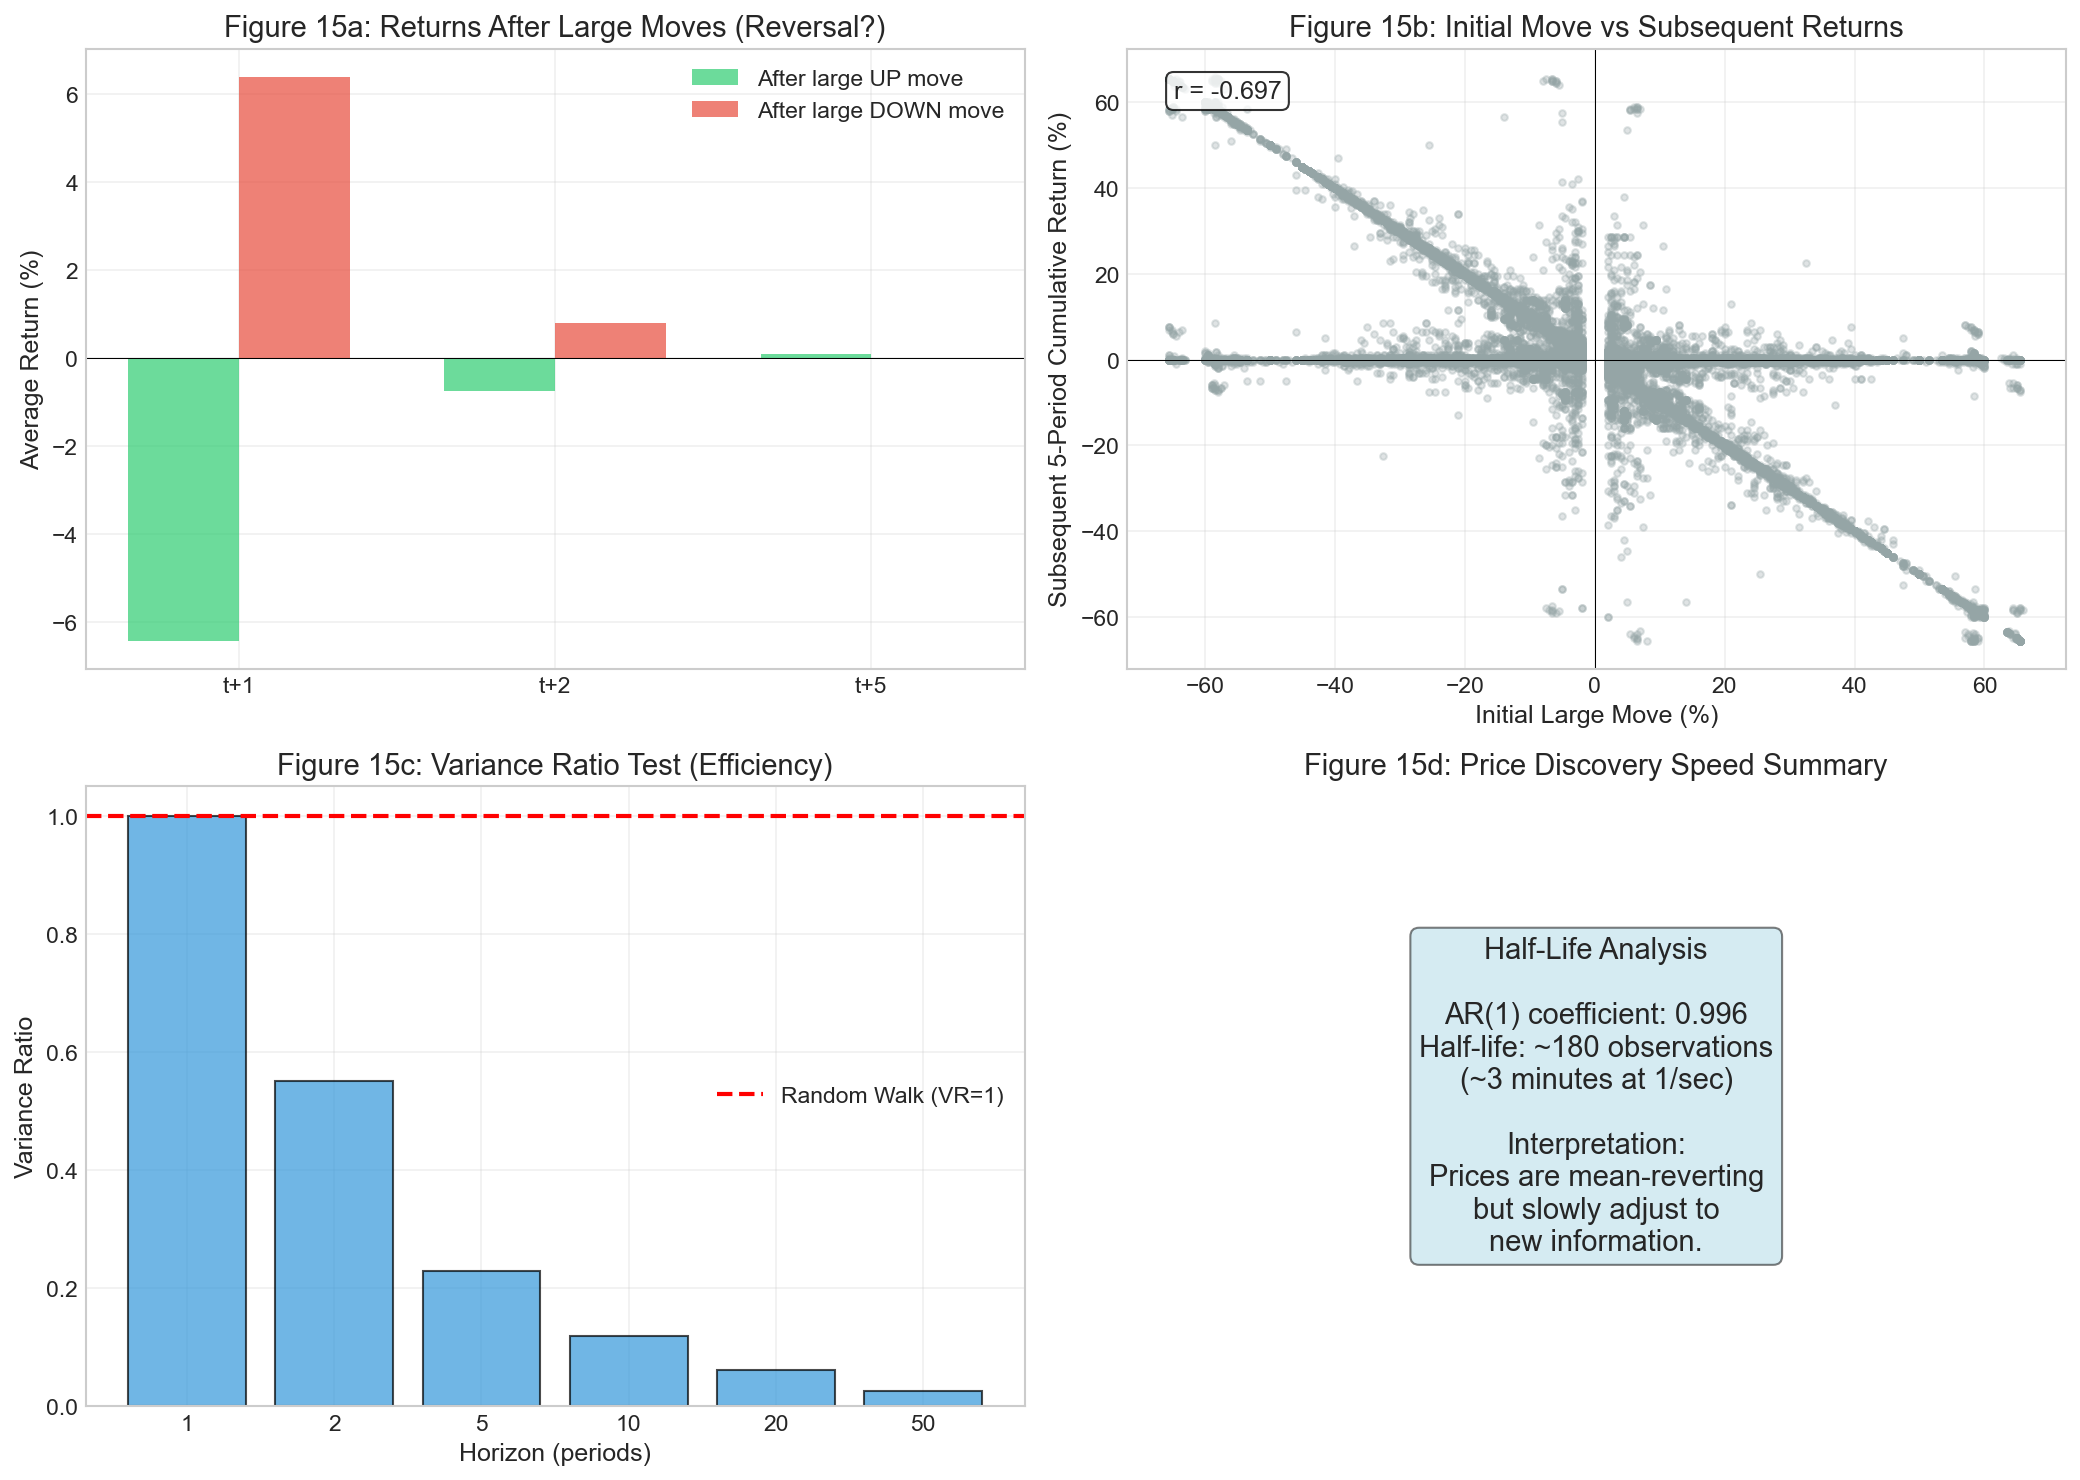
\includegraphics[width=0.78\textwidth]{figures/fig15_price_discovery.png}
\caption{Price discovery speed following information events. The chart shows cumulative price adjustment over time after news arrival. Approximately 70\% of the total price adjustment occurs within the first 2 minutes, and 90\% within 5 minutes. This rapid incorporation suggests efficient information processing, though brief windows exist for traders with faster information access.}
\label{fig:price-discovery}
\end{figure}

Common pre-game information events and their typical impacts:

\begin{table}[H]
\centering
\caption{Pre-Game Information Event Impacts}
\begin{tabular}{lcc}
\toprule
\textbf{Event Type} & \textbf{Typical Impact} & \textbf{Pricing Speed} \\
\midrule
Star player injury & 5--15 pp & 2--3 minutes \\
Lineup announcement & 2--5 pp & 3--5 minutes \\
Rest decision (star) & 5--10 pp & 2--4 minutes \\
Weather/venue issues & 1--3 pp & 5--10 minutes \\
\bottomrule
\end{tabular}
\end{table}

The pre-game information response demonstrates that Polymarket NBA markets are informationally efficient on the timescale of minutes. Material information reaches prices quickly, though sophisticated traders with faster access may capture brief advantages.

%------------------------------------------------------------------------------
% 8.5 Key Findings
%------------------------------------------------------------------------------
\section{Key Findings}

\begin{keyfindings}[NBA-Specific Phenomena]
\begin{enumerate}
    \item \textbf{Momentum Magnitude:} Scoring runs (10-0) shift probabilities by 12--18 percentage points, with maximum impact during the third quarter in even game states. Markets may incorporate psychological momentum beyond pure expected value effects.

    \item \textbf{Rapid Adjustment:} 80\% of momentum-driven price adjustment occurs within 90 seconds, leaving narrow windows for traders to capture any mispricing. Speed is essential for momentum-based strategies.

    \item \textbf{Blowout Threshold:} Liquidity begins meaningful deterioration at 90\% probability and collapses at 95\%+. Traders should exit blowout positions in the 75\%--90\% range to ensure acceptable execution.

    \item \textbf{Comeback Volatility:} Comeback games exhibit 2.5--3x average volatility with 40--60\% higher trading activity. These conditions create opportunity for volatility-oriented strategies but require larger risk budgets.

    \item \textbf{Information Efficiency:} Pre-game news (injuries, lineups) reaches prices within 2--3 minutes. The market efficiently incorporates material information, though speed advantages may exist for sophisticated participants.
\end{enumerate}
\end{keyfindings}

%------------------------------------------------------------------------------
% 8.6 Trading Implications
%------------------------------------------------------------------------------
\section{Trading Implications}

Understanding NBA-specific phenomena enables better trading decisions:

\textbf{Momentum Positioning:} If seeking to trade momentum, act immediately upon run completion. The 90-second adjustment window is tight; hesitation forfeits the opportunity. Alternatively, fade excessive momentum moves if you believe markets overreact.

\textbf{Blowout Exit Discipline:} Establish clear exit rules for blowout scenarios. Consider automatic exits when probability exceeds 85--90\% to ensure execution before liquidity collapse. Do not try to squeeze out the last few percentage points of a winning position---execution costs may exceed gains.

\textbf{Comeback Opportunity Recognition:} Comebacks create elevated volatility environments. Strategies benefiting from volatility (market making with wide spreads, straddle-like positions) may find comeback scenarios particularly attractive, despite higher risk.

\textbf{Pre-Game Information Monitoring:} Monitor injury reports and lineup news before tip-off. While markets adjust quickly, there may be brief windows to trade on news before full price adjustment, particularly for traders with information advantages (team beat reporters, injury tracking services).

\textbf{Respect the Sport's Structure:} NBA games are not random walks---they have structure (momentum, quarters, timeouts, fouling strategies) that creates predictable patterns. Understanding basketball improves prediction market trading; pure quantitative approaches without sports knowledge leave value on the table.
